\documentclass{article}
\usepackage{graphicx}
\usepackage{float}
\usepackage{subcaption}
\usepackage{amsmath}
\graphicspath{{images/}}
\usepackage{caption}
\captionsetup[figure]{position = below,}
\usepackage{listings}
\usepackage{xcolor}
\DeclareCaptionFont{white}{\color{white}}
\DeclareCaptionFormat{listing}{%
  \parbox{\textwidth}{\colorbox{gray}{\parbox{\textwidth}{#1#2#3}}\vskip-4pt}}
\captionsetup[lstlisting]{format=listing,labelfont=white,textfont=white}
\lstset{frame=lrb,xleftmargin=\fboxsep,xrightmargin=-\fboxsep, columns=fullflexible}


\title{Van der Pol equation simulated with Runge-Kutta Algorithm}

\author{Indranil Ghosh\\Jadavpur University\\Physics department\\indranilg49@gmail.com}
\date{\today}
\begin{document}
\maketitle
\begin{abstract}
In this project, a brief overview of Van der Pol Oscillator and the fourth order Runge-Kutta Algorithm are given and the same algorithm has been used to solve and simulate the Van der Pol equation numerically. The equation hasn't an exact, analytic solution, so, needs to be solved numerically. The R codes accompanying the project are available at the end, under the "R Codes" section.
\end{abstract}
\section{Introduction}
Van der Pol Oscillator was originally proposed by the Dutch Electrical Engineer and Physicist, Balthazar Van der Pol in 1920, while working in the \textit{Philips} company. This oscillator is a non-conservative oscillator with non-linear damping, where energy is dissipated at high amplitudes and is generated at low amplitudes. While working with the oscillator, Van der Pol found stable oscillations, which he called the \textit{relaxation oscillations}, which later came to be known as a type of limit cycle in electrical circuits. In electronics, relexation oscillator is a non-linear electronic oscillating circuit that produces non-sinusoidal repeatative wave forms, like square waves or triangular waves.  Van der Pol oscillator has a wide range of applications in Physics, Mathematics, Economics, Biological sciences and Eartth Sciences.
\section{Fourth order Runge Kutta method}
Suppose, the second order initial value equation be,
\begin{center}
$a_0(x)\ddot{y}(x)+a_1(x)\dot{y}(x)+a_2(x)y(x)=F(x)$
\end{center}
with
\begin{center}
$y(x0)=b_0$ and $\dot{y}(x_0)=b1$
\end{center}
We now break this equation into two first order equations, by defining $y=u_1$. So, we have the set of equations, \par
1. $\dot{y}=\dot{u_1}=u_2$, $u_1(x_0)=b_0$\par
2. $\ddot{y}=\dot{u_2}={(F(x) - a_1(x)\dot{y}(x)-a_2(x)y(x)) \over a_0(x)}={(F(x)-a_1(x)u_2-a_2(x)u_1) \over a_0(x)}$, $u_2(x_0)=b_1$ \\ \par
So, \begin{center}
$f1(x, u_1, u_2)=u_2$\\ \par
$f2(x, u_1, u_2)={(F(x)-a_1(x)u_2-a_2(x)u_1) \over a_0(x)}$\\ \par
\end{center}
In vector method, the fourth order Runge-kutta method can be written as,
\begin{center}
$Y_{i}=Y_{i-1}+{(\textbf{K}_1+2\textbf{K}_2+2\textbf{K}_3+\textbf{K}_4) \over 6}, i=1, 2, ...$ \\ \par
\end{center}
Here,
$\textbf{K}_1=\begin{bmatrix}
k_{11}\\
k_{21}\\
\end{bmatrix}$, $\textbf{K}_2=\begin{bmatrix}
k_{12}\\
k_{22}\\
\end{bmatrix}$, $\textbf{K}_3=\begin{bmatrix}
k_{13}\\
k_{23}\\
\end{bmatrix}$ and $\textbf{K}_4=\begin{bmatrix}
k_{14}\\
k_{24}\\
\end{bmatrix}$
Now, 
\begin{center}
$k_{n1}=hf_n(x_i, (Y_1)_i, (Y_2)_i)$, with $n=1, 2$\\ \par
$k_{n2}=hf_n(x_i+{h\over 2}, (Y_1)_i+{k_{11} \over 2}, (Y_2)_i+{k_{21} \over 2})$, with $n=1, 2$\\ \par
$k_{n3}=hf_n(x_i+{h\over 2}, (Y_1)_i+{k_{12} \over 2}, (Y_2)_i+{k_{22} \over 2})$, with $n=1, 2$\\ \par
$k_{n4}=hf_n(x_i+h, (Y_1)_i+k_{13}, (Y_2)_i+k_{23})$, with $n=1, 2$\\ \par
\end{center}
$h$ is the interval between two successive points.
Now, the solutions in the explicit form can be written as, 
\begin{center}
$(Y_1)_i=(Y_1)_{i-1} + {(k_{11}+2k_{12}+2k_{13}+k_{14}) \over 6}$\\ \par
$(Y_2)_i=(Y_2)_{i-1} + {(k_{21}+2k_{22}+2k_{23}+k_{24}) \over 6}$\\ \par
\end{center}
\section{Van der Pol Equation}
The second order non-linear damping differential equation which describes the evolution of the Van der Pol oscillator, with time, is,
\begin{center}
$\ddot{y}-\mu (1-y^2)\dot{y}+y=0$
\end{center}
Here, $y$ is the position coordinate, a function of time and $\mu$ is a constant parameter $>0$, which indicates the nonlinearity and the strength of the damping.\\
\\
Van der Pol equation is a special case of the \textbf{Li\'enard equation}, defined by, 
\begin{center}
$\ddot{y}+f(y)\dot{y}+y=0$
\end{center}
\section{Results for the oscillator without any periodic forcing}
The equation,
\begin{center}
$\ddot{y}-\mu(1-y^2)\dot{y}+y=0$
\end{center}
Let the initial conditions be, $y(t_0)=0.5$ and $\dot{y}(t_0)=0$ and let there be $10^4$ points in the interval $[0, 100]$, so $h=10^{-2}$.\\
\\
We break the equation to a system of two equations by considering,
\begin{center}
$y=y_1$\\ \par
$\dot{y}=\dot{y_1}=y_2$
\end{center}
So, the equation becomes,
\begin{center}
$\dot{y_2}-\mu(1-y_1^2)y_2+y_1=0$
\end{center}
And we get,
\begin{center}
$\dot{y_1}=y_2$ and \\ \par
$\dot{y_2}=\mu(1-y_1^2)y_2-y_1$
\end{center}
So,
\begin{center}
$f_1(t, y_1, y_2)=y_2$ and \\ \par
$f_2(t, y_1, y_2)=\mu(1-y_1^2)y_2-y_1$
\end{center}
Solving these equations by applying fourth order Runge-kutta method yields us the desired results and plots. \\ 
\\
For $0<\mu<1$ the auto oscillations of the Van der Pol oscillator are close to simple harmonic oscillations. \\
\\
\subsection{$\mu=0$}
When $\mu=0$, there is no damipng force and the system conserves energy. Period of oscillation is $2\pi$ with a constant amplitude. The equation becomes, 
\begin{center}
$\ddot{y}+y=0$
\end{center}
This is the equation of simple harmonic equation.
\begin{figure}[H]
\centering 
\noindent\makebox[\textwidth]{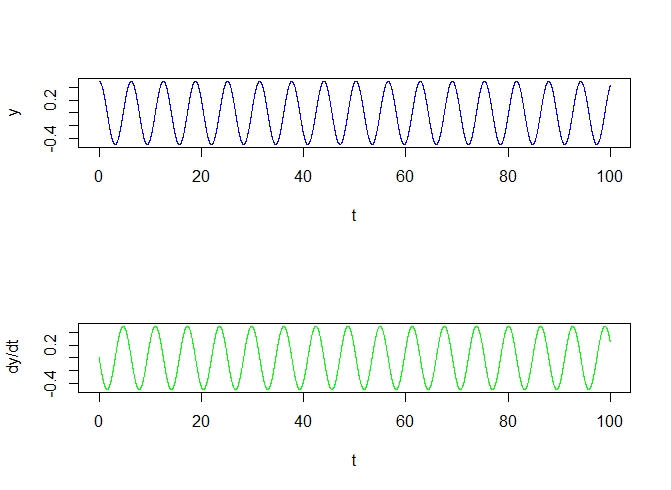
\includegraphics[scale=0.4 ]{mu0}}%
\caption{Change in $y$ and $dy \over dt$  over time, $t$ for $\mu=0$}
\end{figure}
\begin{figure}[H]
\centering 
\noindent\makebox[\textwidth]{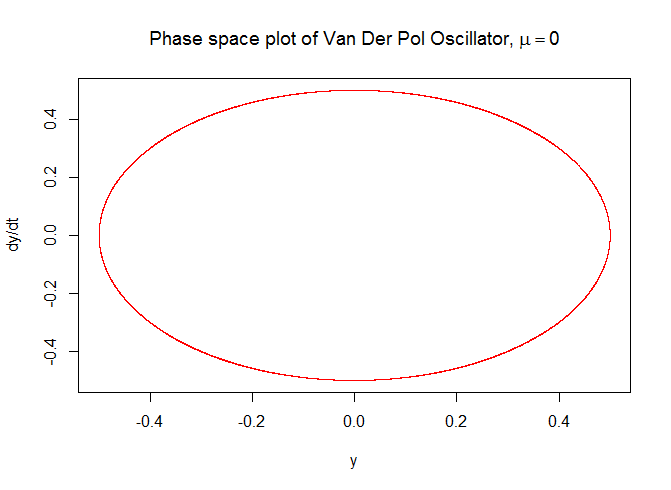
\includegraphics[scale=0.4 ]{phasemu0}}%
\caption{Phase potrait for $\mu=0$}
\end{figure}
With increasing $\mu$, the auto oscillations deviate more and more from harmonic oscillations. The system will enter a limit cycle
\subsection{$\mu=0.1$}
\begin{figure}[H]
\centering 
\noindent\makebox[\textwidth]{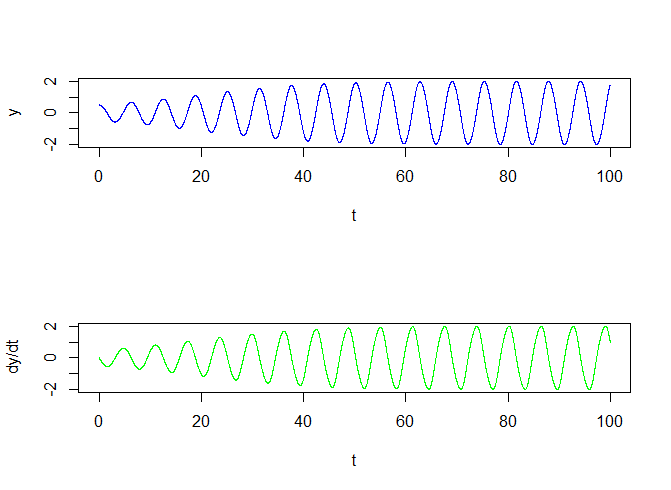
\includegraphics[scale=0.4 ]{mu0point1}}%
\caption{Change in $y$ and $dy \over dt$  over time, $t$ for $\mu=0.1$}
\end{figure}
\begin{figure}[H]
\centering 
\noindent\makebox[\textwidth]{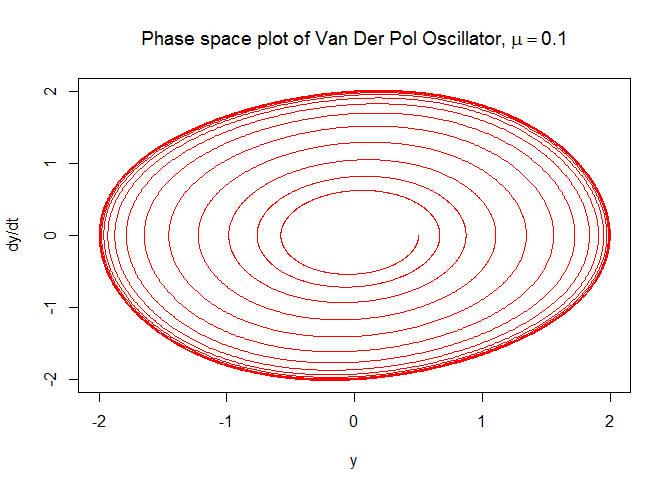
\includegraphics[scale=0.4 ]{phasemu0point1}}%
\caption{Phase potrait for $\mu=0.1$}
\end{figure}
\subsection{$\mu=0.5$}
\begin{figure}[H]
\centering 
\noindent\makebox[\textwidth]{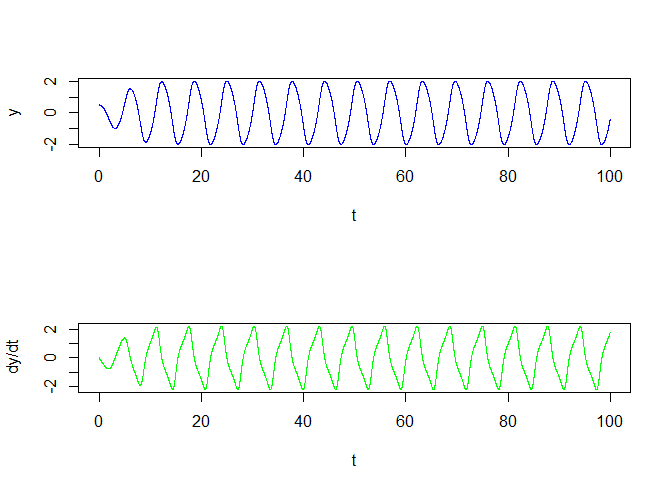
\includegraphics[scale=0.4 ]{mu0point5}}%
\caption{Change in $y$ and $dy \over dt$  over time, $t$ for $\mu=0.5$}
\end{figure}
\begin{figure}[H]
\centering 
\noindent\makebox[\textwidth]{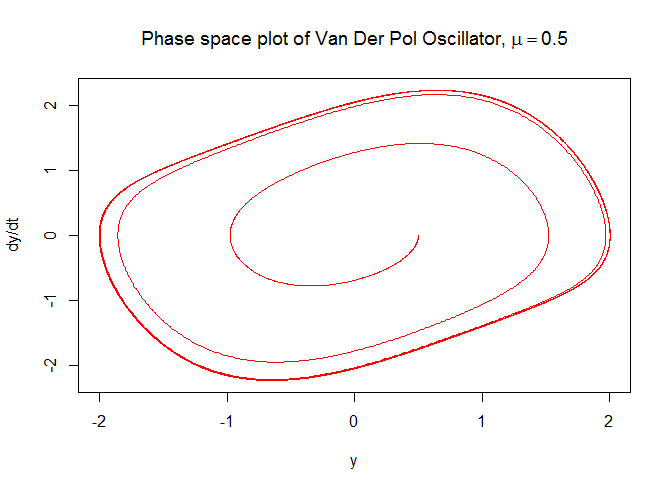
\includegraphics[scale=0.4 ]{phasemu0point5}}%
\caption{Phase potrait for $\mu=0.5$}
\end{figure}
\subsection{$\mu=1$}
\begin{figure}[H]
\centering 
\noindent\makebox[\textwidth]{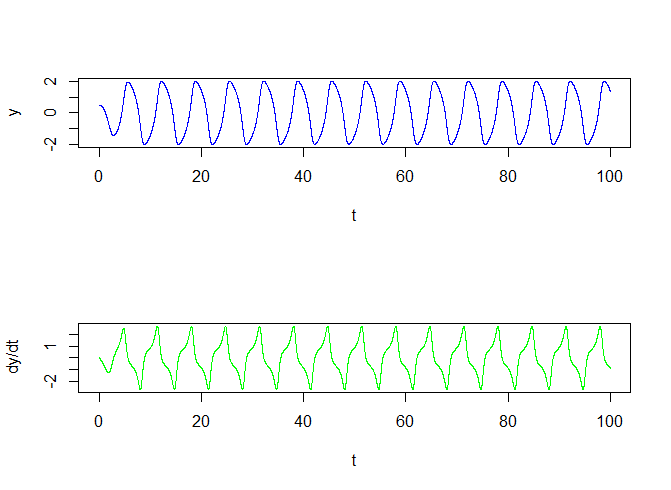
\includegraphics[scale=0.4 ]{mu1}}%
\caption{Change in $y$ and $dy \over dt$  over time, $t$ for $\mu=1$}
\end{figure}
\begin{figure}[H]
\centering 
\noindent\makebox[\textwidth]{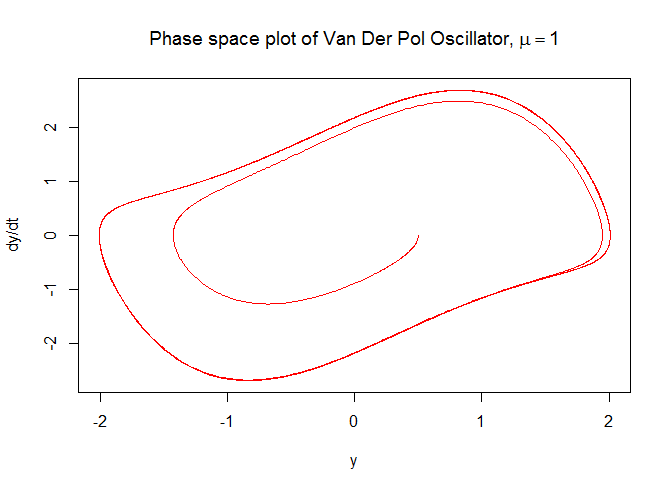
\includegraphics[scale=0.4 ]{phasemu1}}%
\caption{Phase potrait for $\mu=1$}
\end{figure}
Now, we study the behaviour of the oscillator for large lamping, i.e, $\mu>>1$.\\
\\
Van der Pol realised that, his equation for $\mu>>1$, with an electrical circuit consisting of two resistances \textit{R} and \textit{r}, a capacitance \textit{C}, an inductance \textit{L} and a tetrode, the period of oscillation was determined by $\mu=$\textit{RC}. Now, we know, time constant for a R-C circuit, $\tau=$\textit{RC}, he named this oscillation as the \textbf{Relaxation Oscillation}. The characteristics of the Relaxation oscillations are the slow asymptotic behaviour and the sudden discontinuous jump to another value. using few Relaxation oscillations, Van der Pol and Van der Mark modeled the electrical activity of the heart.\\
\\
For large $\mu$, the oscillation is thus described as relaxation oscillation, with period of roughly $1.64\mu$.
\begin{figure}[H]
\centering 
\noindent\makebox[\textwidth]{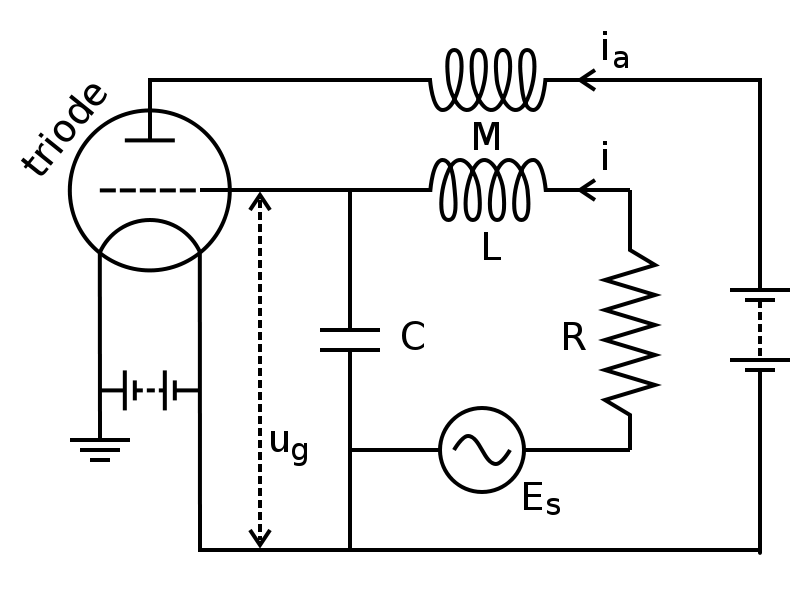
\includegraphics[scale=0.4 ]{circuit}}%
\caption{Figure from Wikipedia}
\end{figure}
\subsection{$\mu=5$}
\begin{figure}[H]
\centering 
\noindent\makebox[\textwidth]{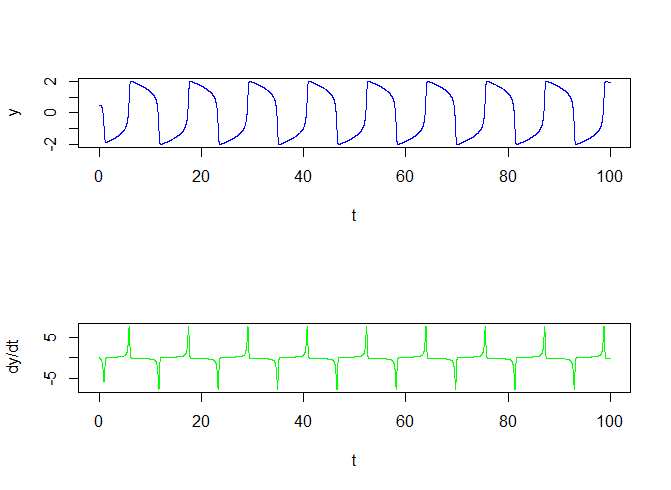
\includegraphics[scale=0.4 ]{mu5}}%
\caption{Change in $y$ and $dy \over dt$  over time, $t$ for $\mu=5$, showing Relaxation Oscillations}
\end{figure}
\begin{figure}[H]
\centering 
\noindent\makebox[\textwidth]{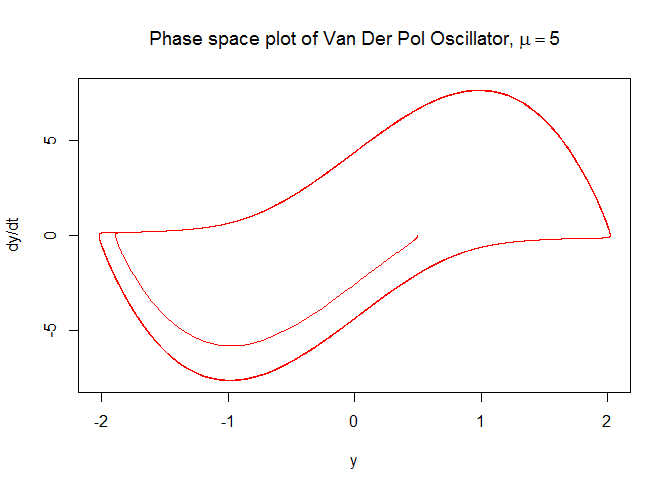
\includegraphics[scale=0.4 ]{phasemu5}}%
\caption{Phase potrait for $\mu=5$}
\end{figure}
\subsection{$\mu=10$}
\begin{figure}[H]
\centering 
\noindent\makebox[\textwidth]{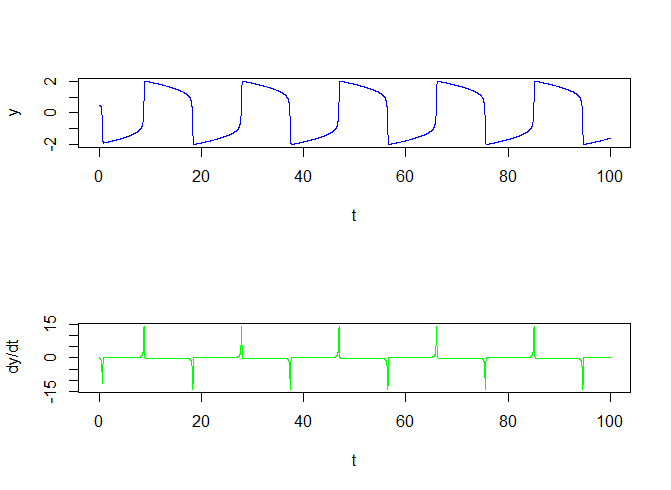
\includegraphics[scale=0.4 ]{mu10}}%
\caption{Change in $y$ and $dy \over dt$  over time, $t$ for $\mu=10$, showing Relaxation Oscillations}
\end{figure}
\begin{figure}[H]
\centering 
\noindent\makebox[\textwidth]{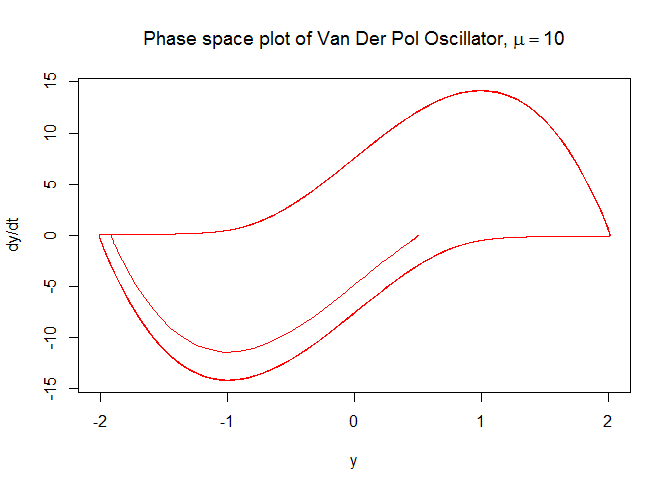
\includegraphics[scale=0.4 ]{phasemu10}}%
\caption{Phase potrait for $\mu=10$}
\end{figure}
\section{Results for the oscillator with the application of periodic forcing}
When the oscillator is acted on by periodic external disturbance, the equation becomes,
\begin{center}
$\ddot{y}-\mu (1-y^2)\dot{y}+y=F\cos{2\pi t \over T_{in}}$
\end{center}
Here, $F$ is the amplitude of the wave function and $\omega={2\pi \over T_{in}}$ is the angular velocity. There exists two frequencies in the system, the frequency of the self oscillation, $\mu$ and the frequency of the periodic forcing. Van der Pol and Van der Mark stated that on application of this external periodic disturbance, some irregular noise was heard, which would be the result of some deterministic chaos. Now, reducing this second order equation similarly as the unforced case, we get two equations,
\begin{center}
$\dot{y_1}=y_2$, and \\ \par
$\dot{y_2}=\mu (1-y^2)y_2-y_1+F\cos{2\pi t \over T_{in}}$
\end{center}
We consider the same initial conditions and the same value of $h$ along with $F=1.2$ and $T_{in}=10$.
\subsection{$\mu=0$}
\begin{figure}[H]
\centering 
\noindent\makebox[\textwidth]{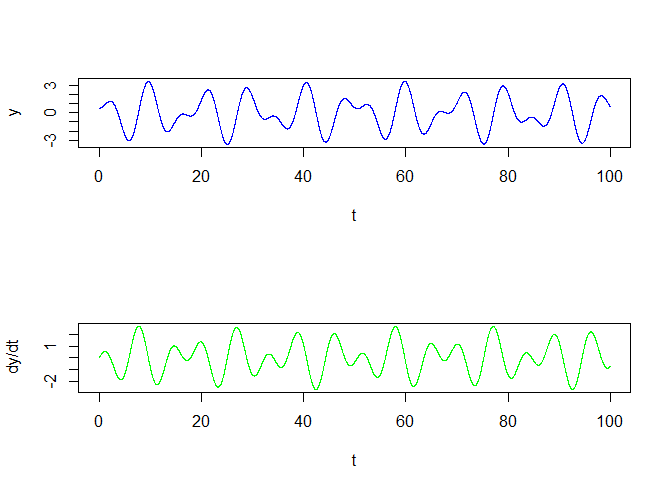
\includegraphics[scale=0.4 ]{fmu0}}%
\caption{Change in $y$ and $dy \over dt$  over time, $t$ for $\mu=0$, with sinusoidal forcing}
\end{figure}
\begin{figure}[H]
\centering 
\noindent\makebox[\textwidth]{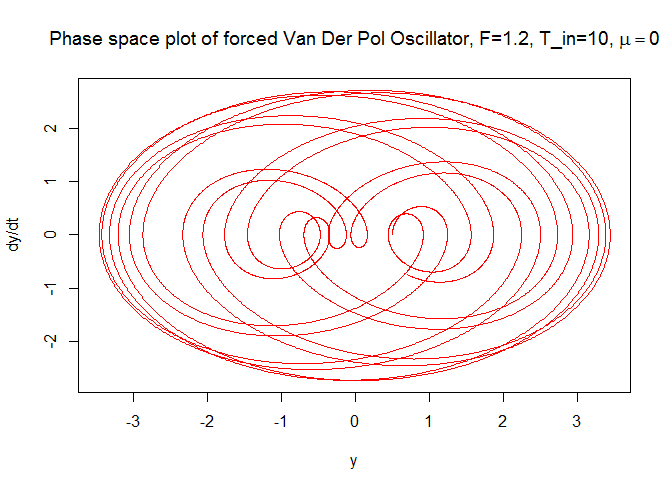
\includegraphics[scale=0.4 ]{fphasemu0}}%
\caption{Phase potrait for $\mu=0$, $F=1.2$ and $T_{in}=10$ with sinusoidal forcing}
\end{figure}
\subsection{$\mu=0.1$}
\begin{figure}[H]
\centering 
\noindent\makebox[\textwidth]{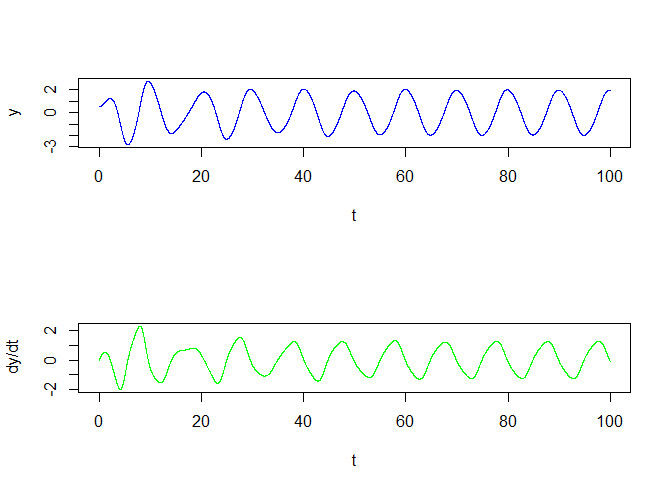
\includegraphics[scale=0.4 ]{fmu0point1}}%
\caption{Change in $y$ and $dy \over dt$  over time, $t$ for $\mu=0.1$, with sinusoidal forcing}
\end{figure}
\begin{figure}[H]
\centering 
\noindent\makebox[\textwidth]{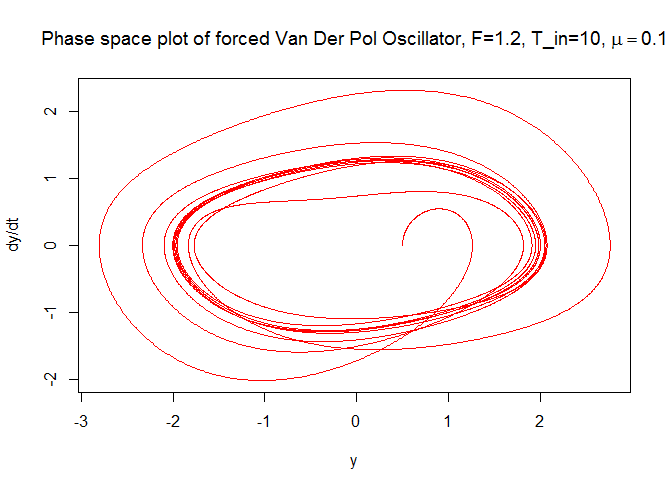
\includegraphics[scale=0.4 ]{fphasemu0point1}}%
\caption{Phase potrait for $\mu=0.1$, $F=1.2$ and $T_{in}=10$ with sinusoidal forcing}
\end{figure}
\begin{figure}[H]
\centering 
\noindent\makebox[\textwidth]{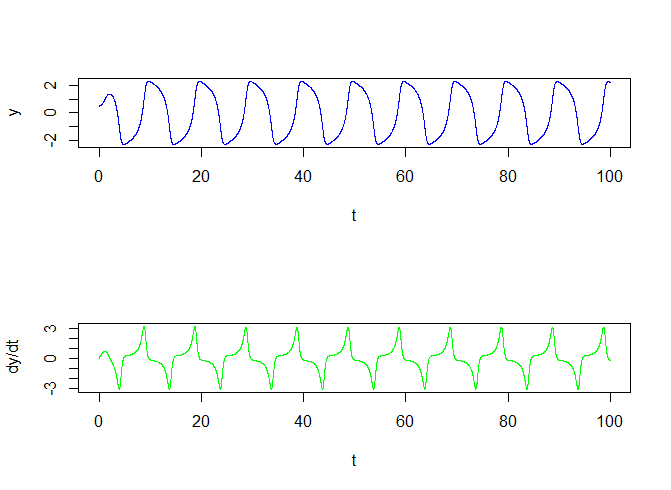
\includegraphics[scale=0.4 ]{fmu1}}%
\caption{Change in $y$ and $dy \over dt$  over time, $t$ for $\mu=1$, with sinusoidal forcing}
\end{figure}
\begin{figure}[H]
\centering 
\noindent\makebox[\textwidth]{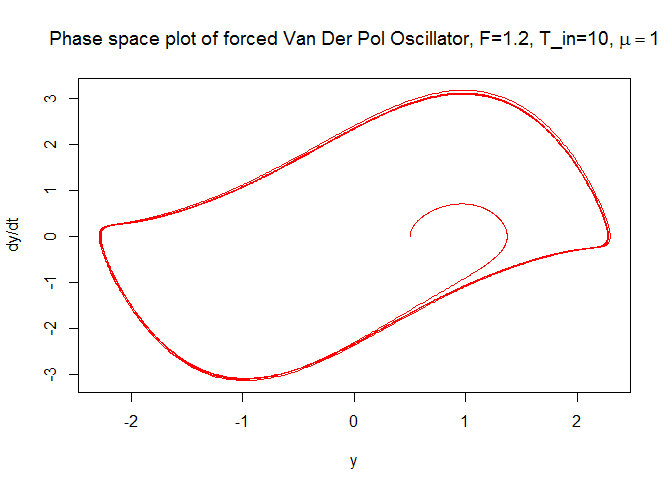
\includegraphics[scale=0.4 ]{fphasemu1}}%
\caption{Phase potrait for $\mu=1$, $F=1.2$ and $T_{in}=10$ with sinusoidal forcing}
\end{figure}
\subsection{$\mu=8.53$}
\begin{figure}[H]
\centering 
\noindent\makebox[\textwidth]{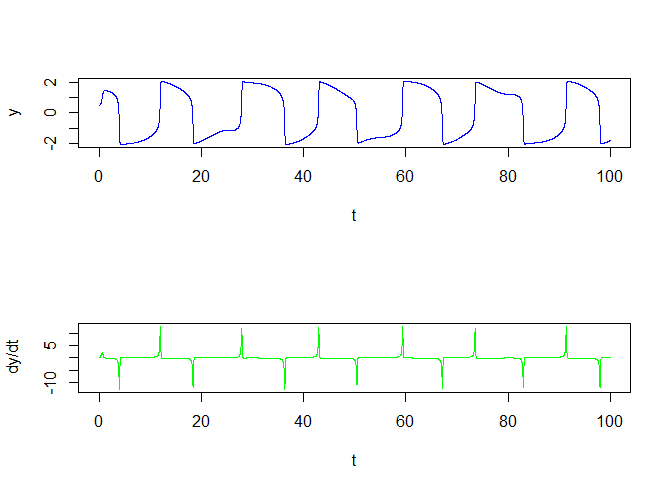
\includegraphics[scale=0.4 ]{fmu8point53}}%
\caption{Change in $y$ and $dy \over dt$  over time, $t$ for $\mu=8.53$, with sinusoidal forcing}
\end{figure}
\begin{figure}[H]
\centering 
\noindent\makebox[\textwidth]{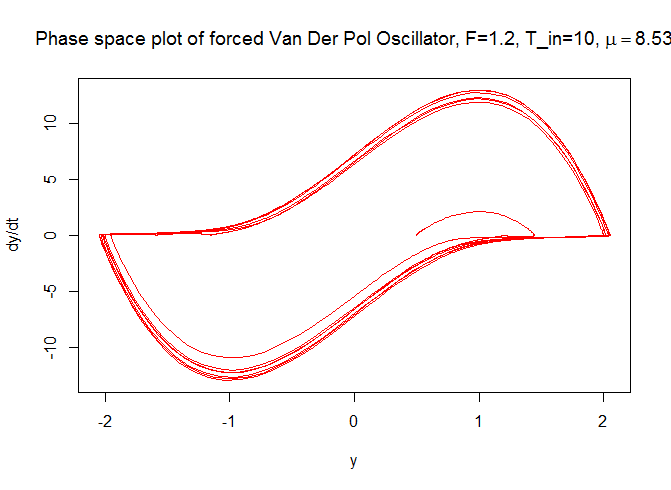
\includegraphics[scale=0.4 ]{fphasemu8point53}}%
\caption{Phase potrait for $\mu=8.53$, $F=1.2$ and $T_{in}=10$ with sinusoidal forcing}
\end{figure}
\subsection{$\mu=10$}
\begin{figure}[H]
\centering 
\noindent\makebox[\textwidth]{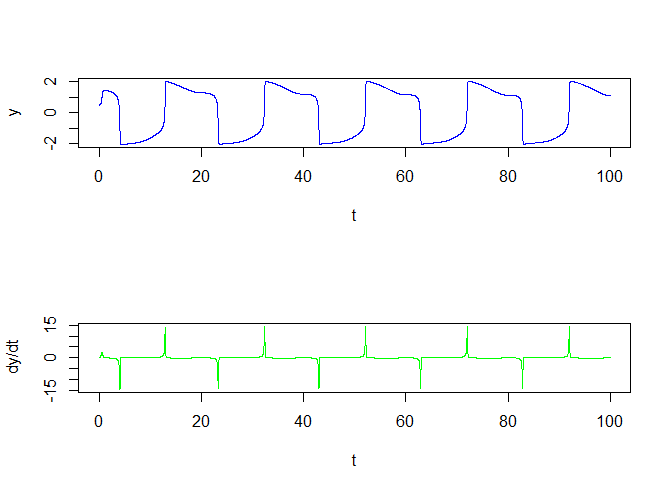
\includegraphics[scale=0.4 ]{fmu10}}%
\caption{Change in $y$ and $dy \over dt$  over time, $t$ for $\mu=10$, with sinusoidal forcing}
\end{figure}
\begin{figure}[H]
\centering 
\noindent\makebox[\textwidth]{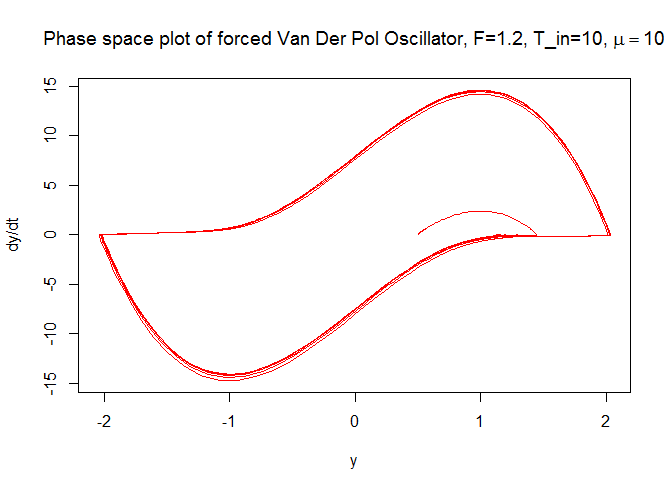
\includegraphics[scale=0.4 ]{fphasemu10}}%
\caption{Phase potrait for $\mu=10$, $F=1.2$ and $T_{in}=10$ with sinusoidal forcing}
\end{figure}
Chaos occurs in the system when the non-linearity becomes sufficiently strong, in the narrow ranges of $\mu$. 
\section{R codes}
\begin{lstlisting}[frame=single, language=R]
#For all the cases we consider, y1_initial=0.5, y2_initial=0, t_initial=0, 
#h=100/10^4, t_final=100

#Determinining the plots of y vs t and dy/dt vs t (Unforced Oscillator)
par(mfrow=c(2, 1))

R <- function(y1_initial, y2_initial, t_initial, h, t_final, mu){
  f1 <- function(t, y1, y2) return(y2)
  f2 <- function(t, y1, y2) return(mu*(1-y1^2)*y2-y1)
  time <- seq(t_initial, t_final, h)
  Y1 <- c(y1_initial)
  Y2 <- c(y2_initial)
  for(i in 2:length(time)) {
    p <- time[i-1]
    q <- Y1[i-1]
    r <- Y2[i-1]
    k11 <- h*f1(p, q, r)
    k21 <- h*f2(p, q, r)
    k12 <- h*f1(p+h/2, q+k11/2, r+k21/2) 
    k22 <- h*f2(p+h/2, q+k11/2, r+k21/2) 
    k13 <- h*f1(p+h/2, q+k12/2, r+k22/2)
    k23 <- h*f2(p+h/2, q+k12/2, r+k22/2)
    k14 <- h*f1(p+h, q+k13, r+k23)
    k24 <- h*f2(p+h, q+k13, r+k23)
    Y1 <- c(Y1, Y1[i-1]+(k11+2*k12+2*k13+k14)/6)
    Y2 <- c(Y2, Y2[i-1]+(k21+2*k22+2*k23+k24)/6)
  }
  plot(time, Y1, type="l", col="blue", ylab="y", xlab="t")
  plot(time, Y2, type="l", col="green", ylab="dy/dt", xlab="t")
}
#for mu=0
R(0.5, 0, 0, 100/10^4, 100, 0)  

#Determing the phase plots (Unforced Oscillator)
par(mfrow=c(1, 1))

Phase <- function(y1_initial, y2_initial, t_initial, h, t_final, mu){
  f1 <- function(t, y1, y2) return(y2)
  f2 <- function(t, y1, y2) return(mu*(1-y1^2)*y2-y1)
  time <- seq(t_initial, t_final, h)
  Y1 <- c(y1_initial)
  Y2 <- c(y2_initial)
  for(i in 2:length(time)) {
    p <- time[i-1]
    q <- Y1[i-1]
    r <- Y2[i-1]
    k11 <- h*f1(p, q, r)
    k21 <- h*f2(p, q, r)
    k12 <- h*f1(p+h/2, q+k11/2, r+k21/2) 
    k22 <- h*f2(p+h/2, q+k11/2, r+k21/2) 
    k13 <- h*f1(p+h/2, q+k12/2, r+k22/2)
    k23 <- h*f2(p+h/2, q+k12/2, r+k22/2)
    k14 <- h*f1(p+h, q+k13, r+k23)
    k24 <- h*f2(p+h, q+k13, r+k23)
    Y1 <- c(Y1, Y1[i-1]+(k11+2*k12+2*k13+k14)/6)
    Y2 <- c(Y2, Y2[i-1]+(k21+2*k22+2*k23+k24)/6)
  }
  obj=list(Mu=mu)
  plot(Y1, Y2, type="l", col="red", ylab="dy/dt", xlab="y",main=
bquote("Phase space plot of Van Der Pol Oscillator," ~ mu==.(obj$Mu)))
}
Phase(0.5, 0, 0, 100/10^4, 100, 0)

#Animating the phase plots
for(mu in  seq(0, 10, 0.25)) {
  Phase(0.5, 0, 0, 100/10^4, 100, mu)
  Sys.sleep(0.09)
}

# for plotting in case of forced oscillator, 
# f2 <- function(t, y1, y2) return(mu*(1-y1^2)*y2-y1+1.2*cos(2*pi*t/10))
\end{lstlisting}
\begin{thebibliography}{9}
\bibitem{knuthwebsite}
\texttt{Numerical Methods by Jain, Iyengar}
\bibitem{knuthwebsite}
\texttt{Scholarpedia, Van der Pol Oscillator, http://www.scholarpedia.org/article/Van der Pol oscillator}
\bibitem{knuthwebsite}
\texttt{Wikipedia,Van der Pol Oscillator, https://en.wikipedia.org/wiki/Van der Pol oscillator}
\bibitem{knuthwebsite}
\texttt{Encyclopedia of Mathematics,Van der Pol equation, https://www.encyclopediaofmath.org/index.php/Van der Pol equation}
\end{thebibliography}
\end{document}